\section{Ausgewählte Absicherungsverfahren}\label{sec:ausgewählte-absicherungsverfahren}

	Für die Identifizierung der Kommunikationspartner
	und damit auch die höherwertige Absicherung von \glspl{api},
	ist es wichtig den Unterschied zwischen den Begrifflichkeiten \gls{authentisierung},
	 \gls{authentifizierung} und \gls{autorisierung} zu verstehen.
	Mit der \gls{authentisierung} weist der Nutzer seine Identität gegenüber des Services/Systems nach.
	Diese Nachweise sind in der Regel Ausweisdokumente,
	oder in der digitalen Welt,
	Passwörter, Muster, Fingerabdrücke, oder Ähnliches.
	In dem darauf folgenden Schritt, der \gls{authentifizierung},
	werden eben diese Nachweise durch eine unabhängige Behörde verifiziert oder falsifiziert,
	was schlussendlich dazu führt,
	dass der Service/das System dem Nutzer Rechte einräumt,
	beziehungsweise Ressourcen freigibt oder verweigert.
	Diesen Schritt bezeichnet man als \gls{autorisierung}.

	Nachfolgend werden zwei Verfahren beschrieben,
	welche zur Absicherung genutzt werden können.
	Diese werden unter anderem in den Kontext der Begrifflichkeiten eingeordnet.

	\subsection{API-Keys}\label{subsec:api-keys}
	Die \gls{api}-Keys eignen sich zur einfachen \gls{autorisierung} eines Clienten
	und werden häufig von Programmen genutzt,
	bei welchen kein direkter Zugriff auf sensible Daten nötig ist.
	Hierzu wird bei beiden Partnern ein gemeinsamer Schlüssel hinterlegt,
	wodurch der Kommunikationspartner identifiziert werden kann.
	Dieser Schlüssel sollte einmalig vergeben werden und wird im Falle von \gls{rest}
	und \gls{http} entweder über die Request-Query bei einem POST-Request
	oder als Header oder \gls{cookie} bei einem GET-Request übergeben.
	Der \gls{webservice} prüft basierend auf dem Schlüssel die genehmigten oder gesperrten Ressourcen
	und wertet anhand der \gls{autorisierung} die Anfrage aus.
	Dieses Verfahren ist stark durch \glspl{manInTheMiddleAngriff} bedroht,
	was unter anderem dazu führt,
	dass es nur unter Benutzung des \gls{https} als sicher gilt,
	da ansonsten der Schlüssel abgefangen und genutzt werden kann.
	\subsection{OAuth 2.0}\label{subsec:oauth-2.0}
	Um einen offenen Standard für die \gls{api}-Zugriffsdelegation zu erstellen,
	wurde im November 2006 eine Initiative gestartet,
	welche zum Ziel haben sollte,
	das OAuth-Protokoll in der Version 1.0 zu entwickeln.
	Ein offener Standard war gewünscht,
	da verschiedene Firmen (z. B. Twitter) bereits eigene Verfahren entwickelt hatten
	und das Beste aus diesen Verfahren zusammengetragen werden sollte,
	um die Implementierung dieser Delegation zu vereinfachen.
	Die Delegation der \gls{authentifizierung} gewinnt zunehmend an Notwendigkeit
	durch immer mehr verschiedene \glspl{webservice} und \webApplications,
	welche ansonsten alle eine eigene Nutzerverwaltung bräuchten.
	OAuth schafft hierbei Abhilfe,
	indem nur gewisse Rechte an die zu nutzende Applikation übertragen werden.
	Die Version OAuth 1.0 wurde also vier Jahre später durch die \gls{ietf} standardisiert\footcite[Vgl.][]{rfc5849}.
	Da diese Version allerdings schwierig zu implementieren war und
	manche Implementierungen sogar Sicherheitslücken aufwiesen,
	wurde im Oktober 2012 die Version 2.0 veröffentlicht\footcite[Vgl.][]{rfc6749}.
	Diese hatte zudem einige andere Vorteile und hat Version 1.0 fast komplett abgelöst,
	da unter anderem auch keine Kompatibilität gegeben ist.
	Im Folgenden wird daher nur auf OAuth 2.0 eingegangen.

	\subsubsection{Rollen}\label{subsubsec:rollen}
		OAuth 2.0 definiert vier verschiedene Rollen,
		welche unter anderem die klassische Client-Server-\gls{authentifizierung} in der Art revolutioniert,
		dass der Client nun in zwei Rollen aufgeteilt wird.

		\myparagraph[resource-owner]{Resource Owner}
		Falls es sich um eine Person handelt wird diese Rolle auch \enquote{end-user} genannt.
		Diese stellt eine Entität dar,
		welche die Fähigkeit hat,
		einem Dritten Zugriff auf ihre geschützten Ressourcen zu gewährleisten.

		\myparagraph[resource-server]{Resource Server}
		Der Resource Server stellt (geschützte) Daten bereit
		und hostet diese.
		Zusätzlich dazu ist dieser ebenfalls in der Lage,
		\accessToken{} zu akzeptieren oder zu verweigern.

		\myparagraph[client]{Client}
		Der Term \client{} erfordert keine besonderen Charakteristiken
		und beschreibt eine (Web)\-Applikation,
		welche Ressourcen beim \hyperref[par:resource-server]{Resource Server} in Vertretung
		des \enquote{end-users} anfragen kann.

		\myparagraph[authorization-server]{Authorization Server}
		Um \nameref{subsubsec:token} für die \gls{autorisierung} beim \hyperref[par:resource-server]{Resource Server} zu bekommen,
		wird der \hyperref[par:authorization-server]{\authorizationServer} genutzt.
		Dieser kann \nameref{subsubsec:token} erstellen, verschicken und validieren.

	\subsubsection{Token}\label{subsubsec:token}
		Die Sicherheit im Zugriff auf geschützte Ressourcen
		kann bei \nameref{subsec:oauth-2.0} durch \enquote{Token} gewährleistet werden.
		Am häufigsten kommen sogenannte \enquote{Bearer-Token} zum Einsatz.

		\myparagraph[access-token]{Access Token}
		Diese Token werden genutzt,
		um Zugangsdaten eines \hyperref[par:resource-owner]{Resource Owners},
		spezifische Bereiche und die Dauer des Zugriffs
		für einen \clienten{} verschlüsselt bereitzustellen.
		Die Darstellung erfolgt als String
		und ist üblicherweise undurchsichtig für den \clienten.
		Zudem können sie je nach Sicherheitsrichtlinien des Servers in der Darstellung und Verschlüsselung variieren.

		\myparagraph[refresh-token]{Refresh Token}
		Refresh Token sind optional und -- wie der Name sagt -- dafür da,
		die bereits ausgestellte Berechtigung zu erneuern.
		Der \client{} nutzt dieses Token nur im Austausch
		mit dem \hyperref[par:authorization-server]{\authorizationServer},
		um ein neues \accessToken{} zu erhalten.
		Hiermit kann die Sicherheit dieses Protokolls zusätzlich verstärkt werden,
		falls die Lebensdauer des \accessTokens{} kurz gewählt wird und
		der \client{} für Anfragen häufig über das \refreshToken{} ein neues \accessToken{} beantragen muss.

		\vspace{1em}

		\begin{figure}[h]
			\centering
			\pgfplotsset{width=.8\textwidth}
			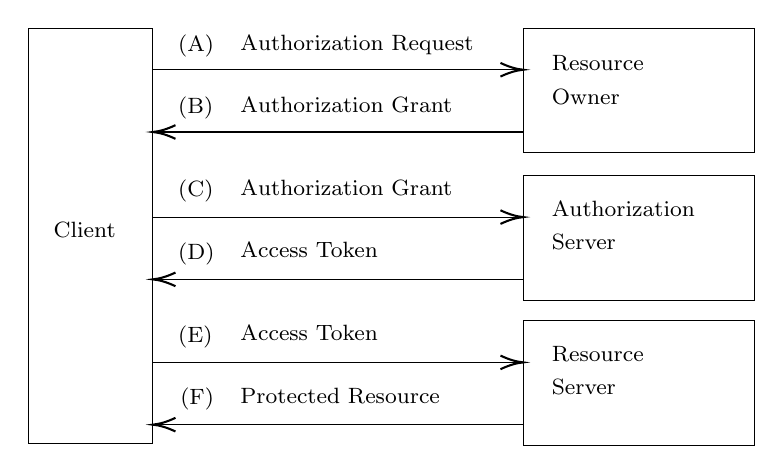
\begin{tikzpicture}[x=0.75pt,y=0.75pt,yscale=-1,xscale=1]
%uncomment if require: \path (0,241); %set diagram left start at 0, and has height of 241

%Shape: Rectangle [id:dp9112141025931051]
	\draw   (10,10) -- (70,10) -- (70,210) -- (10,210) -- cycle ;
%Shape: Rectangle [id:dp2466907608570026]
	\draw   (248.46,10) -- (360,10) -- (360,70) -- (248.46,70) -- cycle ;
%Shape: Rectangle [id:dp667913005920042]
	\draw   (248.46,81) -- (360,81) -- (360,141) -- (248.46,141) -- cycle ;
%Shape: Rectangle [id:dp38178981445269944]
	\draw   (248.46,151) -- (360,151) -- (360,211) -- (248.46,211) -- cycle ;
%Straight Lines [id:da8122455913426612]
	\draw    (70,30) -- (246.46,30) ;
	\draw [shift={(248.46,30)}, rotate = 180] [color={rgb, 255:red, 0; green, 0; blue, 0 }  ][line width=0.75]    (10.93,-3.29) .. controls (6.95,-1.4) and (3.31,-0.3) .. (0,0) .. controls (3.31,0.3) and (6.95,1.4) .. (10.93,3.29)   ;
%Straight Lines [id:da5648885701594799]
	\draw    (70,101) -- (246.46,101) ;
	\draw [shift={(248.46,101)}, rotate = 180] [color={rgb, 255:red, 0; green, 0; blue, 0 }  ][line width=0.75]    (10.93,-3.29) .. controls (6.95,-1.4) and (3.31,-0.3) .. (0,0) .. controls (3.31,0.3) and (6.95,1.4) .. (10.93,3.29)   ;
%Straight Lines [id:da09731573656651382]
	\draw    (70,171) -- (246.46,171) ;
	\draw [shift={(248.46,171)}, rotate = 180] [color={rgb, 255:red, 0; green, 0; blue, 0 }  ][line width=0.75]    (10.93,-3.29) .. controls (6.95,-1.4) and (3.31,-0.3) .. (0,0) .. controls (3.31,0.3) and (6.95,1.4) .. (10.93,3.29)   ;
%Straight Lines [id:da4634800234879517]
	\draw    (248.46,201) -- (72,201) ;
	\draw [shift={(70,201)}, rotate = 360] [color={rgb, 255:red, 0; green, 0; blue, 0 }  ][line width=0.75]    (10.93,-3.29) .. controls (6.95,-1.4) and (3.31,-0.3) .. (0,0) .. controls (3.31,0.3) and (6.95,1.4) .. (10.93,3.29)   ;
%Straight Lines [id:da41475583524040527]
	\draw    (248.46,131) -- (72,131) ;
	\draw [shift={(70,131)}, rotate = 360] [color={rgb, 255:red, 0; green, 0; blue, 0 }  ][line width=0.75]    (10.93,-3.29) .. controls (6.95,-1.4) and (3.31,-0.3) .. (0,0) .. controls (3.31,0.3) and (6.95,1.4) .. (10.93,3.29)   ;
%Straight Lines [id:da5062439224159696]
	\draw    (248.46,60) -- (72,60) ;
	\draw [shift={(70,60)}, rotate = 360] [color={rgb, 255:red, 0; green, 0; blue, 0 }  ][line width=0.75]    (10.93,-3.29) .. controls (6.95,-1.4) and (3.31,-0.3) .. (0,0) .. controls (3.31,0.3) and (6.95,1.4) .. (10.93,3.29)   ;

% Text Node
	\draw (21,102) node [anchor=north west][inner sep=0.75pt]   [align=left] {{\footnotesize Client}};
% Text Node
	\draw (261,22) node [anchor=north west][inner sep=0.75pt]   [align=left] {{\footnotesize Resource}\\{\footnotesize Owner}};
% Text Node
	\draw (261,92) node [anchor=north west][inner sep=0.75pt]   [align=left] {{\footnotesize Authorization}\\{\footnotesize Server}};
% Text Node
	\draw (261,162) node [anchor=north west][inner sep=0.75pt]   [align=left] {{\footnotesize Resource}\\{\footnotesize Server}};
% Text Node
	\draw (111,12) node [anchor=north west][inner sep=0.75pt]  [font=\footnotesize] [align=left] {{\footnotesize Authorization Request}};
% Text Node
	\draw (111,42) node [anchor=north west][inner sep=0.75pt]  [font=\footnotesize] [align=left] {{\footnotesize Authorization Grant}};
% Text Node
	\draw (111,82) node [anchor=north west][inner sep=0.75pt]  [font=\footnotesize] [align=left] {{\footnotesize Authorization Grant}};
% Text Node
	\draw (111,112) node [anchor=north west][inner sep=0.75pt]  [font=\footnotesize] [align=left] {{\footnotesize Access Token}};
% Text Node
	\draw (111,152) node [anchor=north west][inner sep=0.75pt]  [font=\footnotesize] [align=left] {{\footnotesize Access Token}};
% Text Node
	\draw (111,182) node [anchor=north west][inner sep=0.75pt]  [font=\footnotesize] [align=left] {{\footnotesize Protected Resource}};
% Text Node
	\draw (81,12) node [anchor=north west][inner sep=0.75pt]  [font=\footnotesize] [align=left] {(A)};
% Text Node
	\draw (81,42) node [anchor=north west][inner sep=0.75pt]  [font=\footnotesize] [align=left] {(B)};
% Text Node
	\draw (81,82) node [anchor=north west][inner sep=0.75pt]  [font=\footnotesize] [align=left] {(C)};
% Text Node
	\draw (81,112) node [anchor=north west][inner sep=0.75pt]  [font=\footnotesize] [align=left] {(D)};
% Text Node
	\draw (81,152) node [anchor=north west][inner sep=0.75pt]  [font=\footnotesize] [align=left] {(E)};
% Text Node
	\draw (82,182) node [anchor=north west][inner sep=0.75pt]  [font=\footnotesize] [align=left] {(F)};


\end{tikzpicture}

			\caption[OAuth 2.0 Abstrakter Protokoll Fluss]
			{OAuth 2.0 Abstrakter Protokoll Fluss\label{fig:oauthAbstractFlow}\\Quelle: \fullcite{rfc6749}}
		\end{figure}

	\subsubsection{Abstrakter Protokollfluss}\label{subsubsec:abstrakter-protokollfluss}
		\vref{fig:oauthAbstractFlow} zeigt den allgemeinen abstrakten Ablauf
		einer \gls{autorisierung} mit OAuth 2.0 und ist wie folgt dargestellt:

		\begin{compactenum}[(A)]
			\item Der \hyperref[par:client]{Client} beantragt die \gls{autorisierung}
			des \hyperref[par:resource-owner]{Resource Owners}.
			Diese Anfrage kann entweder direkt an den \hyperref[par:resource-owner]{Resource Owner} gestellt werden
			oder besser indirekt durch den \hyperref[par:authorization-server]{\authorizationServer} als Vermittler.

			\item Der \hyperref[par:resource-owner]{Resource Owner} antwortet mit einer
			\glslink{autorisierung}{Autorisierungsgenehmigung},
			welche eine aus vier zugelassenen Typen sein kann,
			die jeweils abhängig von den unterstützten Typen
			des \hyperref[par:authorization-server]{\authorizationServers} sind.

			\item Der \client{} fordert ein \accessToken{}
			in Kombination mit der vorher erhaltenen \glslink{autorisierung}{Autorisierungsgenehmigung}
			beim \hyperref[par:authorization-server]{\authorizationServer} an.

			\item Der \hyperref[par:authorization-server]{\authorizationServer} \glslink{authentisierung}{authentisiert}
			den \clienten,
			validiert die \glslink{autorisierung}{Autorisierungsgenehmigung} und
			gibt ein \accessToken{} heraus.

			\item Der \client{} fragt die Ressource beim \hyperref[par:resource-server]{\resourceServer} an
			und \glslink{authentifizierung}{authentifiziert} sich mit dem \accessToken.

			\item Der \hyperref[par:resource-server]{\resourceServer} prüft das \nameref{subsubsec:token}
			im Zusammenspiel mit dem \hyperref[par:authorization-server]{\authorizationServer} und
			erteilt Zugriff auf die angefragte Ressource.

		\end{compactenum}

		\vspace{1em}

		\begin{figure}[h]
			\centering
			\pgfplotsset{width=.8\textwidth}
			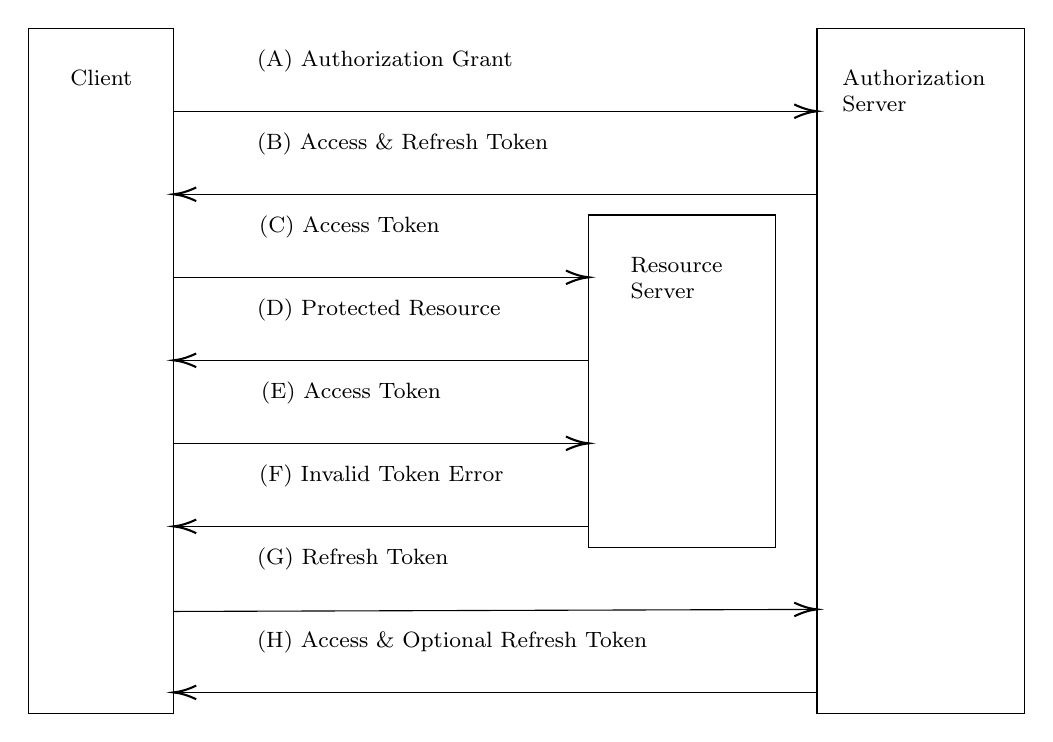
\begin{tikzpicture}[x=0.75pt,y=0.75pt,yscale=-1,xscale=1]
%uncomment if require: \path (0,408); %set diagram left start at 0, and has height of 408

%Shape: Rectangle [id:dp13364236400121876]
	\draw   (10,10) -- (80,10) -- (80,340) -- (10,340) -- cycle ;
%Shape: Rectangle [id:dp8790780704634384]
	\draw   (390,10) -- (490,10) -- (490,340) -- (390,340) -- cycle ;
%Shape: Rectangle [id:dp4236723129691826]
	\draw   (280,100) -- (370,100) -- (370,260) -- (280,260) -- cycle ;
%Straight Lines [id:da25292034726719925]
	\draw    (80,50) -- (388,50) ;
	\draw [shift={(390,50)}, rotate = 180] [color={rgb, 255:red, 0; green, 0; blue, 0 }  ][line width=0.75]    (10.93,-3.29) .. controls (6.95,-1.4) and (3.31,-0.3) .. (0,0) .. controls (3.31,0.3) and (6.95,1.4) .. (10.93,3.29)   ;
%Straight Lines [id:da8910220128583559]
	\draw    (390,90) -- (82,90) ;
	\draw [shift={(80,90)}, rotate = 360] [color={rgb, 255:red, 0; green, 0; blue, 0 }  ][line width=0.75]    (10.93,-3.29) .. controls (6.95,-1.4) and (3.31,-0.3) .. (0,0) .. controls (3.31,0.3) and (6.95,1.4) .. (10.93,3.29)   ;
%Straight Lines [id:da8301570060257315]
	\draw    (80,130) -- (278,130) ;
	\draw [shift={(280,130)}, rotate = 180] [color={rgb, 255:red, 0; green, 0; blue, 0 }  ][line width=0.75]    (10.93,-3.29) .. controls (6.95,-1.4) and (3.31,-0.3) .. (0,0) .. controls (3.31,0.3) and (6.95,1.4) .. (10.93,3.29)   ;
%Straight Lines [id:da33179095828439187]
	\draw    (280,170) -- (82,170) ;
	\draw [shift={(80,170)}, rotate = 360] [color={rgb, 255:red, 0; green, 0; blue, 0 }  ][line width=0.75]    (10.93,-3.29) .. controls (6.95,-1.4) and (3.31,-0.3) .. (0,0) .. controls (3.31,0.3) and (6.95,1.4) .. (10.93,3.29)   ;
%Straight Lines [id:da04499082975726765]
	\draw    (80,210) -- (278,210) ;
	\draw [shift={(280,210)}, rotate = 180] [color={rgb, 255:red, 0; green, 0; blue, 0 }  ][line width=0.75]    (10.93,-3.29) .. controls (6.95,-1.4) and (3.31,-0.3) .. (0,0) .. controls (3.31,0.3) and (6.95,1.4) .. (10.93,3.29)   ;
%Straight Lines [id:da7604152906927255]
	\draw    (280,250) -- (82,250) ;
	\draw [shift={(80,250)}, rotate = 360] [color={rgb, 255:red, 0; green, 0; blue, 0 }  ][line width=0.75]    (10.93,-3.29) .. controls (6.95,-1.4) and (3.31,-0.3) .. (0,0) .. controls (3.31,0.3) and (6.95,1.4) .. (10.93,3.29)   ;
%Straight Lines [id:da8975431920651942]
	\draw    (80,291) -- (388,290.01) ;
	\draw [shift={(390,290)}, rotate = 179.82] [color={rgb, 255:red, 0; green, 0; blue, 0 }  ][line width=0.75]    (10.93,-3.29) .. controls (6.95,-1.4) and (3.31,-0.3) .. (0,0) .. controls (3.31,0.3) and (6.95,1.4) .. (10.93,3.29)   ;
%Straight Lines [id:da4986555462596063]
	\draw    (390,330) -- (82,330) ;
	\draw [shift={(80,330)}, rotate = 360] [color={rgb, 255:red, 0; green, 0; blue, 0 }  ][line width=0.75]    (10.93,-3.29) .. controls (6.95,-1.4) and (3.31,-0.3) .. (0,0) .. controls (3.31,0.3) and (6.95,1.4) .. (10.93,3.29)   ;

% Text Node
	\draw (29,29) node [anchor=north west][inner sep=0.75pt]  [font=\footnotesize] [align=left] {{\footnotesize Client}};
% Text Node
	\draw (401.02,29) node [anchor=north west][inner sep=0.75pt]  [font=\footnotesize] [align=left] {{\footnotesize Authorization}\\{\footnotesize Server}};
% Text Node
	\draw (119,19) node [anchor=north west][inner sep=0.75pt]  [font=\footnotesize] [align=left] {{\footnotesize (A) Authorization Grant}};
% Text Node
	\draw (119,59) node [anchor=north west][inner sep=0.75pt]  [font=\footnotesize] [align=left] {{\footnotesize (B) Access \& Refresh Token}};
% Text Node
	\draw (120,99) node [anchor=north west][inner sep=0.75pt]  [font=\footnotesize] [align=left] {{\footnotesize (C) Access Token}};
% Text Node
	\draw (119,139) node [anchor=north west][inner sep=0.75pt]  [font=\footnotesize] [align=left] {{\footnotesize (D) Protected Resource}};
% Text Node
	\draw (121,179) node [anchor=north west][inner sep=0.75pt]  [font=\footnotesize] [align=left] {{\footnotesize (E) Access Token}};
% Text Node
	\draw (120,219) node [anchor=north west][inner sep=0.75pt]  [font=\footnotesize] [align=left] {{\footnotesize (F) Invalid Token Error}};
% Text Node
	\draw (299,119) node [anchor=north west][inner sep=0.75pt]  [font=\footnotesize] [align=left] {{\footnotesize Resource}\\{\footnotesize Server}};
% Text Node
	\draw (119,259) node [anchor=north west][inner sep=0.75pt]  [font=\footnotesize] [align=left] {{\footnotesize (G) Refresh Token}};
% Text Node
	\draw (119,299) node [anchor=north west][inner sep=0.75pt]  [font=\footnotesize] [align=left] {{\footnotesize (H) Access \& Optional Refresh Token}};


\end{tikzpicture}

			\caption[OAuth 2.0 Refreshing an Expired Access Token]
			{OAuth 2.0 Refreshing an Expired Access Token\label{fig:oauthrefreshToken}\\Quelle: \fullcite{rfc6749}}
		\end{figure}

	\subsubsection{Beantragung eines Refresh Tokens}\label{subsubsec:beantragung-eines-refresh-tokens}
		Um das vorher genannte \accessToken{} neu beantragen zu können,
		da meistens eine Gültigkeitsdauer gesetzt ist,
		wird -- wie in \vref{fig:oauthrefreshToken} gezeigt --
		zusammen mit dem \refreshToken{} ein neues \accessToken{} beantragt.
		Der Ablauf ist wie folgt:

		\begin{compactenum}[(A)]
			\item Wie bei der ersten Beantragung eines \accessTokens{}
			schickt der \client{} eine \glslink{autorisierung}{Autorisierungsanfrage}
			an den \hyperref[par:authorization-server]{\authorizationServer}.

			\item Der \hyperref[par:authorization-server]{\authorizationServer} antwortet daraufhin
			sowohl mit einem \accessToken{} als auch mit einem \refreshToken.

			\item Der \client{} beantragt die geschützten Daten beim \hyperref[par:resource-server]{\resourceServer}
			in Kombination mit dem \accessToken.

			\item Falls das \accessToken{} valide ist,
			wird der Request mit den angefragten Daten beantwortet.

			\item Die Schritte (C) und (D) werden so lange wiederholt,
			bis die Lebensdauer des \accessTokens{} ausgelaufen ist.
			Wenn der \client{} dies weiß,
			wird direkt zum Schritt (G) gesprungen,
			andernfalls wird ein erneuter Request abgesetzt.

			\item Da das \accessToken{} nun ungültig ist,
			wird vom \hyperref[par:resource-server]{\resourceServer} ein \enquote{Invalid Token Error} zurückgegeben.

			\item Der \client{} beantragt ein neues \accessToken{}
			beim \hyperref[par:authorization-server]{\authorizationServer},
			indem dieser das \refreshToken{} zeigt und sich \glslink{autorisierung}{autorisiert}.

			\item Wenn die Validierung des \refreshTokens{} geklappt hat,
			erteilt der \hyperref[par:authorization-server]{\authorizationServer} dem \clienten{}
			ein neues \accessToken,
			sowie optional auch ein neues \refreshToken.

		\end{compactenum}